% ----------------------------------------------------------
% Tecnologias Envolvidas
% ----------------------------------------------------------
\chapter{Tecnologias Envolvidas} \label{cha:tecnologias}

Aqui, descreva as tecnologias, linguagens de programação, frameworks, bibliotecas e ferramentas utilizadas no desenvolvimento do projeto. Explique por que cada uma foi escolhida e como elas contribuem para o sucesso do projeto. Inclua também informações sobre bancos de dados, servidores e outras tecnologias relevantes.

\section{Título da Seção SECUNDÁRIA}



Exemplo de gráfico:



\begin{figure}[H]
\renewcommand{\figurename}{Gráfico}	
\caption*{ \label{graf2}Gráfico 2 – Distribuição do número de matrículas por etapas da 
educação básica município de Avaré – 2014}
	\begin{center}
	    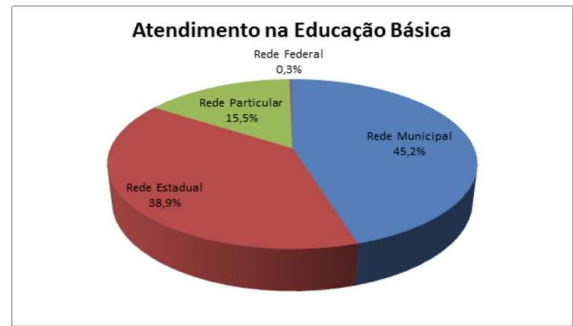
\includegraphics[scale=1.0]{imagens/grafs_1.png}
	\end{center}
	\legend{Fonte: Secretaria Municipal de Educação de Avaré (2014). }

\end{figure}

\renewcommand{\figurename}{Figura}	

\setcounter{secnumdepth}{4}

\titleformat{\paragraph}
{\normalfont\normalsize}{\theparagraph}{1em}\emph{}
\titlespacing*{\paragraph}
{0pt}{3.25ex plus 1ex minus .2ex}{1.5ex plus .2ex}


\subsection{Título da seção terciária}

Exemplo de figura:

\begin{figure}[H]
	\caption{\label{fig_arranjo}Arranjo produtivo local da banana orgânica.}
	\begin{center}
	    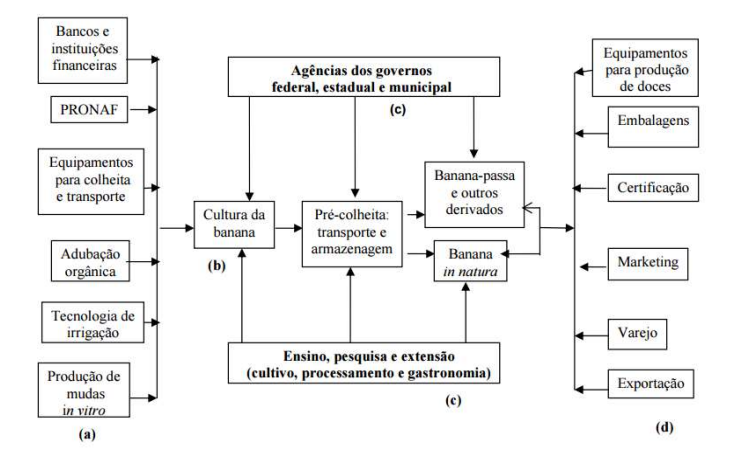
\includegraphics[scale=1.0]{imagens/fig_exemplo.png}
	\end{center}
	\legend{Fonte: \cite{limaarranjo}}
\end{figure}


